\chapter{Introduction}
\label{chap:intro}

\makeatletter
\newenvironment{chapquote}[2][2em]
{\setlength{\@tempdima}{#1} \def\chapquote@author{#2} \parshape 1
  \@tempdima \dimexpr\textwidth-2\@tempdima\relax \itshape}
{\par\normalfont\hfill--\
\chapquote@author\hspace*{\@tempdima}\par\bigskip}
\makeatother

\begin{chapquote}{Morgan Freeman in {\em Transcendence (2014 film)}}
  ``Geo-locating suspects in real time? I've never seen anything like
it.''
\end{chapquote}

The ultimate goal of image understanding is to transfer visual
signals (images/videos) into abstract symbolic descriptions of the
world which are helpful for decision making.
However, understanding images is a not trivial task for machines.
In order to handle various complicated scenarios, researchers divide
image understanding into different computer vision tasks: pedestrian
detection for autonomous driving, face recognition for security
system, and image retrieval for image searching engines.

For many applications, knowing when, where, and in which direction a
picture was taken is important to understand the world. However, most
images does not carry such information. Our thesis focuses on
developing algorithms to estimate this information.
We refer to the task of estimating these properties as {\em
geo-calibration}.
Most recent work of geo-calibration focus on deterministic systems
\todo{citations}, 
which have some drawbacks: 1) they can not model the inherent
uncertainties from images of ambiguous scenes, and 2) without a proper
modeling of the uncertainty, subsequent processing can yield overly
confident predictions. To address these problems, we propose to build
probabilistic models for camera geo-calibration.

We also show that learning to geo-calibrate a camera allows us to
implicitly learn to understand the content of the scene.
As an essential part of scene understanding, how to extract image
features is an important problem being studied for decades.  In
recent years, learning based approaches for image feature extraction
like convolutional neural networks have drawn a lot of attention due
to the fact that they do not need expert knowledge about the target
data. However, most of these feature learning methods require large
quantity of manually labeled data sets.  In this thesis, we presented
alternative ways to learn high-level image features when the
manually labeled data is either insufficient or absent.

\section{Background}
For a better understanding of our work, we would like to introduce
some related computer vision concepts in this section before the
discussion of the main topics.

\subsection{Geo-Calibration of Outdoor Images}
Automatic geo-calibration of outdoor images continues to grow in
importance as a direct result of the increasing amount of imagery
available via the Internet. Solving this problem is of great value
for a wide variety of fields, with potential applications ranging from
the forensic sciences~\cite{stylianou13jane} to environmental
monitoring~\cite{zhang2012mining}. Conceptually the geo-calibration
task includes: identifying the camera pose ({\em pose estimation}),
the camera geographic location ({\em geo-localization}), and the time
when the query image was captured ({\em time estimation}).

\begin{itemize}[noitemsep]

\item \textbf{Pose Estimation:}
Pose estimation includes estimating the camera yaw, pitch, and roll
angles, $(\theta_{yaw}, \theta_{pitch}, \theta_{roll})$ from a
image. In the context of geo-calibration, the yaw angle
$\theta_{yaw}$ is referred to as the geographic orientation angle of
the camera.
%
Li et al.~\cite{li2012worldwide} exploit geo-registered 3D points
clouds to estimate camera pose.
Vo \etal~\cite{vo2016localizing} propose a geo-localization network
that can regress the geo-orientation angle of the camera.
Agarwal \etal~\cite{agarwal2015metric} keep track of the camera pose
changes by matching SIFT~\cite{lowe1999object} feature points detected
between the input image and Google Street View panoramas.
%
Horizon line detection is an essential step for some pose
estimation algorithms, because horizon lines are closely related to
camera pitch and roll angles.
%If the camera focal length is known, one can compute the camera pitch
%and roll angle from the horizon line.
Collins and Weiss~\cite{unitsphere1990} formulate horizon line
detection as a statistical estimation problem on the Gaussian Sphere,
which is similar to the geometry we use.  More recent work has
explored the use of dual space~\cite{alignment2014,dualspace2013}
representations. Among the clustering-based approaches, Xu et
al.~\cite{kitware2013} improve this pipeline by introducing a new
point-line consistency function that models errors in the line segment
extraction step.
\newline

\item \textbf{Geo-Localization:}
The task of geo-localization estimates the geographic location, $(lat,
lon)$, of the camera from the input image or video frames.
%
As an important step of geo-localization, extracting
location-dependent features from image data has drawn a great detail
of attention from the vision community~\cite{jacobs07geolocate,
jacobs11geolocate, jacobs08geoorient}. The common trend amongst these
methods is that they take advantage of a large dataset of
geo-referenced images. Hays and Efros~\cite{hays2008im2gps} use a
data-driven scene matching approach to localize a query image using a
large dataset of geo-tagged images.  Doersch
\etal~\cite{doersch2012what} extract location-dependent features that
capture the relative appearance differences of large cities.  Lin et
al.~\cite{lin2013cross} localize a ground-level image by learning the
relationship between pairs of ground and aerial images \footnote{In
the context of our thesis, we do not distinguish between satellite
imagery and aerial imagery} of the same location. Other techniques
focus on urban environments and infer location using local image
descriptors~\cite{schindler2008detecting,snavely2006photo}.  Many
other cues exist, such as the
skyline~\cite{baatz2012large,ramalingam2009geolocalization}, sky
appearance~\cite{lalonde2010sun,workman2014rainbow}, and
shadows~\cite{junejo2008estimating,wu2010geo}.
\newline

\item \textbf{Time Estimation:}
The goal of time estimation is to estimate the time when the input
image was captured. Depending on the application, the scale of a
time estimator outputs may range from year to hour.
%
Matzen and Snavely~\cite{matzen2014scene} predict
timestamps for photos by matching against a time-varying
reconstruction of a scene.  Hill~\cite{hill1994elephant} estimate the
time of the day by measuring the light intensity profiles captured by
cameras. Methods are proposed to date the
year book photos by analyzing human
appearance~\cite{salem2016face2year,ginosar2015century}. Lee
\etal~\cite{linking2015iccp} find visual paterns in the buildings,
relate them to certain time periods.
\newline

\end{itemize}

In conclusion, most of the geo-calibration algorithms we mention above
relies on finding visual cues from the input images. The development
of these algorithms require strong human expertise about the data,
thus can only be applied in limited scenarios. Therefore, researchers
need new methodologies in order to make the development of
geo-calibration algorithms more efficient.

\subsection{Deep Learning in Geo-Calibration}
In recent years, deep neural networks (DNNs) were proven to be
extremely successful in many computer vision areas. 
It is widely accepted that DNNs have excellent performance in
high-level visual feature learning.
This valuable ability provides researchers powerful tools to
solve the challenging geo-calibration tasks.
Weyand and Kostrikov \etal~\cite{planet} propose a convolutional
neural network (CNN) to predict the geographic location of the input
image. Walch \etal~\cite{walch2017image} aggregate learned CNN
features with LSTM to generate global image representation for camera
localization.  Studies about camera pose
estimation~\cite{zhai2016horizon, workman2016horizon,
hold2017perceptual} has been done by identifying the horizon line with
CNNs (one can derive the camera roll and pitch angles from the horizon
line position giving the camera focal length).

Closely related to camera geo-calibration, problems of identifying
camera intrinsics using deep neural networks have also been studied.
Workman \etal~\cite{workman2015deepfocal} develop a CNN to estimate
the camera focal length. Kendall \etal~\cite{kendall2015convolutional}
propose a neural network that can identify 6-DOF camera parameters for
specific scenes.

These geo-calibration methods make the predictions directly out of
DNNs.  There is another big category of geo-calibration methods that
use aerial imagery as geo-registered database, which we will introduce
in the following section.

\subsection{Ground-to-Aerial Geo-Calibration}
Data-driven scene matching approaches are commonly used in
geo-calibration.
When localizing a camera, data-driven algorithms search for k-nearest
neighbors of the query image in a database of the geo-tagged imagery.
To reduce the work of querying, the searching process is usually
carried out in feature space of applicable number of  
dimensions~\cite{im2gps, li2010location,zamir2010accurate}.
However, due to limited accuracies of GPS signals and the biased
distribution of human population, geo-tagged ground-level images
collected from smart devices are usually noisy and sparse in
geographic space. To achieve better geo-calibration results, we
need alternative image resources with more accurate geographic tags
and more complete spatial coverage.

Benefited from the fast growing monitoring satellite and drone markets,
the geo-tagged aerial imagery becomes more publicly accessible
than ever. Aerial imagery downloading services like
Microsoft Bing Map provide aerial images of various
resolutions, which cover most areas of the world with accurate
geographic registration, making aerial imagery a rich source for
reference databases. We refer to geo-calibration
methods which use the aerial imagery for geographic reference as
ground-to-aerial geo-calibration. Data used for ground-to-aerial
geo-calibration is referred to as cross-view pairs.
A cross-view pair consists of a ground image and an aerial image at
the same location, and but not necessarily aligned in orientation.

Recent work on ground-to-aerial
geo-calibration~\cite{lin2013cross,lin2015learning,workman2015geocnn,workman2015wide}
has shown that convolutional neural networks are efficient for extracting
features from geo-tagged aerial imagery that can be matched to
features extracted from the ground imagery.  Vo
\etal~\cite{vo2016localizing} extend this line of work, demonstrating
improved geo-localization performance by applying an auxiliary loss
function to regress the ground-level camera orientation with respect
to the aerial image. Hu and Feng \etal~\cite{mh2018cvm} achieve the
state-of-the-art performance in geo-localization by extracting
cross-domain global features using the
NetVLAD~\cite{arandjelovic2016netvlad} technique.

The key for the success of these ground-to-aerial geo-calibration
methods is to learn descriptive features good for ground-to-aerial
imagery matching. In the following section, we will show how to use
geo-calibration information to learn useful features.

\subsection{Geo-Calibration for Feature Learning}

Manually engineering visual features is a common practice for many
computer vision tasks. One of the successful example of manually
engineered feature is the SIFT feature~\cite{lowe1999object}.
In recent years, automatic feature engineering has drawn a lot
of attention. Compared to the manual feature
engineering, automatic feature engineering approaches allow to learn
useful features without strong expert knowledge about the data. Among
these approaches, deep neural networks are wildly accepted as good
tools to learn high-level image representations.  The most commonly
used approach for deep feature learning is full supervision, which
usually requires large number of manual
annotations~\cite{yosinski2014transferable,zhou2016learning,wen2016discriminative}.
Unfortunately, such data is not always available for certain tasks or
needs to invest a huge amount of human labors to create.
In contrast, unlabeled data is often plentiful (\ie cellphone photos
in Instagram or Youtube videos).

To exploit these unlabeled data, recent work has explored
self-supervision methods (sometimes referred to as unsupervised learning or
pretext tasks) for training deep neural networks that capture useful
visual representations~\cite{doersch2015unsupervised,pathak2016context}. 
These methods typically
exploit some known quantity of the data, like pixel color values, to
avoid expensive manual annotation.
By learning these quantities associated with the data, one
can obtain useful features of the image.
For example, Zhang et al.~\cite{zhang2016colorful} show how image
colorization (synthesizing colors for a grayscale image) is a powerful
pretext task for learning visual representations. Pathak et
al.~\cite{pathak2017learning} exploit low-level motion-based grouping
cues for unsupervised feature learning.  
%
As new learning technique that addresses the lack of massive amounts
of labeled data, domain adaptation forces the feature generating model
to adapt another feature domain so that it improves the performance
when dealing with new input
data~\cite{fernando2013unsupervised,fernando2015joint,saenko2010adapting,wang2016actions,tinghui2016flow}.
Duan \etal~\cite{duan2012learning} propose to learn a linear
projection to transfer from the source feature subspace to the target
subspace. Sohn \etal~\cite{sohn2017unsupervised} improve the
performance of video face recognition using an adversarial-based
approach to adapt the network to unlabeled video imagery.

So far, we have explained four important related computer vision
concepts. In the following section, we are going to discuss our main
contributions in this thesis.

\section{Main Contributions}

\begin{figure}
  \centering
  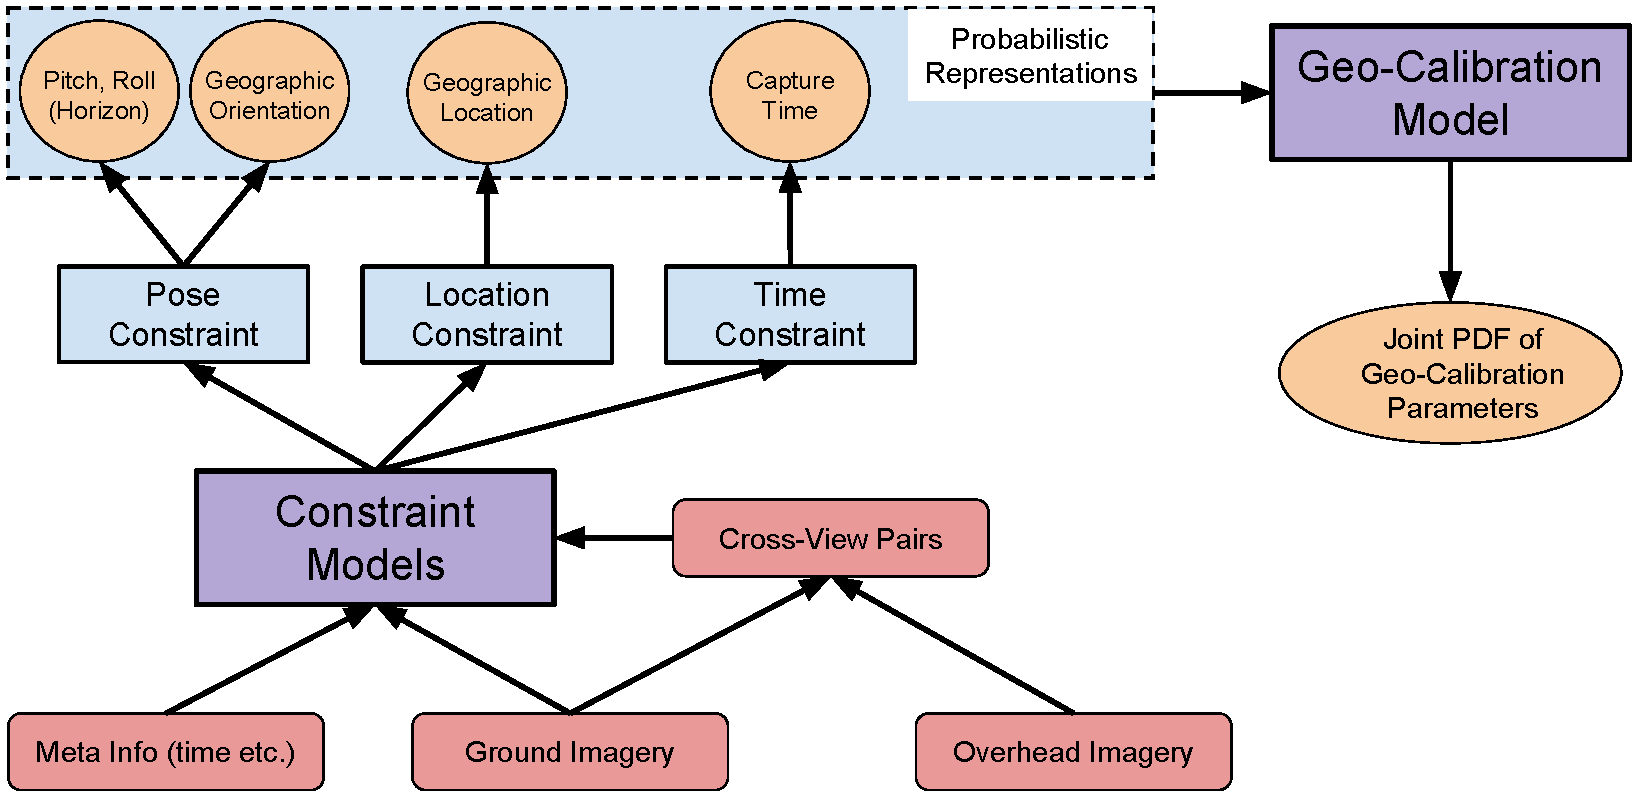
\includegraphics[width=\linewidth]{introduction/architecture}
  \caption{A simplified flowchart of our approach. The algorithm
inputs (images, time and manual annotations) are fed to different
constraint models which work as constraint functions. 
The probabilistic distribution over complete geo-calibration
parameters are then simulated jointly by fusing these constraint
functions in a general model for geo-calibration.}
  \label{fig:intro:architecture}
\end{figure}

We make contributions in three main areas: 1) we proposed a general
probabilistic model to jointly estimate the geo-calibration
parameters, 2) we decomposed the full geo-calibration into several
partial geo-calibration tasks, each of which provides a strong
constraint function that fits into the general model, and 3) we show
that learning to geo-calibrate a camera is a useful pretext for image
feature learning.
 
The first two contributions make our main approach. Our
algorithm feeds inputs (images, time and manual annotations) to
different constraint functions. Then
we fuse these constraint functions to simulate the joint distribution
over the complete geo-calibration parameters. We present the flowchart of
our approach in \figref{intro:architecture}.
%
Furthermore, we also explore to learning image features
and geo-calibrating cameras simultaneously.  We believe that camera
poses, geographic locations and image capture times are closely
related to image representations. 
Based on the belief that visual features which abstract the image
contents are the necessary for solving the geo-calibration tasks, we
designed neural networks to learn useful visual features by
geo-calibrating cameras. Our work provide new ways for automatic
feature learning.


\subsection{General Probabilistic Model for Geo-Calibration}
We design a general model to estimate the probability over all
geo-calibration parameters. First, we model the process of projecting
from the scene at given location, time, and in given camera pose.
%This the appearance of the image frame are determined by the pin-hole
%model and the geographic location of the camera.
We use a scoring function to measure the ``fitness'' between these
geo-calibration parameters and the appearance of the image. 
The scoring function is proportional to the probability distribution
over the geo-calibration parameters, but the denominator is unknown. We
then propose a Markov Chain Monte Carlo (MCMC) sampling approach to
approximate the underlying probability distribution.
Our model is flexible that it is able to contribute different
constraint functions to the scoring function. The details of this model
can be found in \chapref{mcmc}.

\subsection{Developing Constraint Functions}
In the general model, we define the scoring function as a weighted
summation of a series of constraint functions.
In the rest of the work, we focus on developing good constraint
functions for different sets of geo-calibration parameters. 
A constraint function outputs a score or probability for some given
geo-calibration parameters conditional on the input image.

\begin{itemize}[noitemsep]
  \item \textbf{Constraint for Camera Pose:}
  In this constraint, we model the camera roll and pitch angles.
  Assuming the intrinsic parameters are known, camera roll and pitch
  angles can be derived from the horizon line position on the image.
  Compared to directly detecting the camera pose, identifying horizon
  line is easier because it is reflected by the scene layout.
  In our work, we create a new method using CNN to estimate the
  prior distribution over the horizon line. We assign a probability to
  each horizon candidate sampled from the prior distribution by
  measuring their consistences with detected vanishing points. We
  present the algorithm details in \chapref{fasthorizon}.  \newline

  \item \textbf{Constraint for Time and Location:}
  In this work, we estimate the probability over the
  capture time and the camera geographic location given the input image.
  Our network has two branches which predict the image
  capture time and the geographic location simultaneously.
  For time estimation, our network is able to predict the
  joint distribution over the month of the year and the UTC hour of the
  day when the input image has been captured.
  For coarse camera geo-localization, We provide two approaches to
  obtain the probability distribution over the camera geographic
  location. Most straightforwardly, our network outputs the discrete
  distribution over the geographic location of the camera. Better
  results can be procured with the image capture time as auxiliary input
  (if it is known).  We present the algorithm details in
  \chapref{whenwhere}.
  \newline

  \item \textbf{Constraint for Location and Orientation:}
  In our previous method, we present that our algorithm can estimate
  the discrete camera location. The predictions are only approximate
  due to the limitation of the algorithm. In this
  work, we propose a ground-to-aerial geo-calibration method that can
  further refine the prediction results and estimate the
  camera geo-orientation with overhead imagery.
  %
  We designed a network that can jointly learn the semantic layout of
  the aerial image and its projection to the ground-level perspective.
  When computing the value of constraint function, feed the aerial
  image of a given location and orientation set to the network. 
  By comparing the aerial-to-ground layout with the real layout of the
  ground image, we are able to measure the consistency of these two as
  the value of our constraint function.
  We present the algorithm details in \chapref{crosstransf}.
  \newline

\end{itemize}


\subsection{Geo-Calibration for Feature Learning}
Our methods also provide another way to dealing with the challenges of
lacking manual annotations during DNN training. By learning to
geo-calibrate a camera, we believe the networks are able to learn
high-level image representations. This belief comes from the fact that
the geo-calibration information of a camera encodes semantic
information because it is closely related to the appearances of the
scene.
We explore two types of learning techniques for high-level feature
extraction: 1) semantic segmentation of the aerial imagery with
ground-level annotations which is plentiful, and 2) geo-temporal
features with automatically annotated geographic locations and time.

\begin{itemize}[noitemsep]
  \item \textbf{Ground-to-Aerial Feature Learning:}
  Most current machine learning methods study problems involving the
  ground imagery. There exist many annotated dataset of the ground
  imagery while much fewer of the aerial imagery. 
  In \chapref{crosstransf}, we proposed a
  method to learn to semantically segment aerial images with only
  ground-level annotations. Our method exploits the spatial
  correspondences between images in cross-view pairs. 
  In this work, we try to transfer the semantic knowledge from the
  ground domain to the aerial domain by identifying their latent
  geometric correspondences. Similar to {\em
  Reprojection Losses}~\cite{garg2016unsupervised,
  godard2017unsupervised,zhou2017unsupervised, yan2016perspective}
  which have been successfully applied in monocular depth estimation,
  our network learns geometric projection from aerial to ground, and
  to semantically segment the aerial images jointly.
  \newline

  \item \textbf{Geo-Temporal Feature Learning:}
  In \chapref{whenwhere}, we demonstrate that our algorithm is able to
  learn geo-temporal image representations with geographic locations and
  capture time which are automatically captured by smart devices.
  Our work is most similar to Li and Snavely~\cite{li2018learning},
  who propose an approach for learning intrinsic images by observing
  image sequences with varying illumination over time. While their
  targets are reflectance and shading images of the scene, we consider
  two novel pretext tasks, time and location estimation.
  By learning to predict the geographic location and capture time of
  the query image, our network learns to extract geo-temporal features
  from the image.

\end{itemize}
